\documentclass[
	parskip=half,10pt,
	numbers= noenddot, % enddot -> Ebenen mit Punkt abschließen -> 1.1., noenddot -> ohne Punkt
	toc=flat, % TOC in Tabellenform (bei langen Überschrtiften verwenden)
	oneside,
	twocolumn,
	]{scrartcl}



\usepackage[T1]{fontenc} % verwende Type 1 - Zeichensatz
\usepackage{libertine}
\usepackage[scaled=0.78]{beramono} %Schreibmaschinenschrift
\usepackage{microtype}
\usepackage[utf8]{inputenc}
\usepackage[english]{babel} % internationale Sprachunterstützung



\usepackage{amsmath}
\usepackage{amssymb}
\usepackage{amsthm}
\usepackage{tabularx}
\usepackage{booktabs}
\usepackage{longtable}
\usepackage{rotating} % Rotationen, Reflexionen, ...
\usepackage{multido} % Wiederholungen
\usepackage{wrapfig}
\usepackage{todonotes}
\usepackage{siunitx} %\si units
\usepackage{units}
\usepackage{icomma} %keine Leerzeichen nach Komma im mathmode
\usepackage[numbers,sort]{natbib}
\usepackage{babelbib} %deutsche bibliographie
\usepackage{multirow}
\usepackage{rotating}
\usepackage{url}

\usepackage{tikz}
\usepackage{float}
\usepackage{pgfplots}
%\pgfplotsset{compat=1.8}
\usepackage{caption}
\usepackage{graphicx}
\usepackage{subcaption} %für subfigures
\captionsetup{labelfont={bf,sf},format = plain, textfont=sf}
%\usepackage{asymptote}
\usepackage{ragged2e}
\usepackage[bottom]{footmisc}
\usepackage{csquotes} %Anführungszeichen
\usepackage[ngerman]{varioref} % Zum komfortablen Verlinken



\usepackage{geometry}
\geometry{a4paper,lmargin=2.5cm, rmargin=2.5cm, tmargin=2.5cm, bmargin=3cm, marginparwidth=3cm, marginparsep=1em}


\usepackage{fancyhdr}
\pagestyle{fancy}
\renewcommand\footrulewidth{0.5pt}
\fancyhf{}
\lhead{\leftmark}

\fancyfoot{}
\rfoot{\thepage}
\lfoot{Till Kolster \& Lukas Schmidt}


\usepackage{layout}

\usepackage[%draft
linkbordercolor=blue,
colorlinks,
linkcolor=blue,
linktocpage,
linktoc=all]{hyperref} % IMMER AM ENDE

%\setkomafont{subparagraph}{\mdseries\itshape}
\setcounter{secnumdepth}{3}%Bis zu welcher Ebene nummeriert werden soll. 
\setcounter{tocdepth}{2}%Bis zu welcher Tiefe ins TOC soll.

%%%%%EIGENE DEFINITIONEN%%%%%

\newcolumntype{Y}{>{\RaggedRight\hspace{0pt}} X }
\newcommand\Grad{$^\circ$}
\newcommand\HAND{\marginnote{\Large\vreflectbox{\ding{43}}}\xspace}%\newcommand\Name{Befehlsdifinition}
\newcommand\MPAR[1]{
\marginnote[\RaggedLeft#1]{\RaggedRight#1}}
% \hspace{0pt} entspricht dem ersten (nicht sichtbaren) Wort
\newcolumntype{P}[1]{>{\RaggedRight\hspace{0pt}}p{#1}}
\newcolumntype{R}{>{\tiny}r}

\pgfmathdeclarefunction{gauss}{4}{%
  \pgfmathparse{#1*exp(-((x-#2)^2)/(2*#3^2))+#4}%
}


\title {Rayleigh-Scattering}
\author {Till Kolster \thanks{Freie Universität Berlin} \and Lukas Schmidt \thanks{Freie Universität Berlin}}


\begin{document}

\begin{titlepage}

\vspace*{-2cm}

\vspace{6cm}
\begin{center}
\huge \bfseries
Fortgeschrittenen-Praktikum -- Gamma-Spektroskopie

\vspace{0.5cm}
\large \bfseries
\today

\vspace{1.5cm}

\large\normalfont von

\bigskip
\textbf{Till Kolster \& Lukas Schmidt}

\bigskip
Tutor: Dr. Katayoun Gharagozloo-Hubmann

\vspace{3cm}

\parbox{0.8\linewidth}{%
\textit{Kleiner Text}}


\end{center}
\end{titlepage}

\section{Einleitung}

Radiokativer Zerfall feststellen

\section{Theoretische Grundlagen}

\subsection{Kernzerfälle}

$\alpha \beta \gamma$ Zerfälle, Nuklidkarte, Herkunft von Strahlung/Komponenten

\subsection{Photoeffekt}

\subsection{Compton-Streuung}

\subsection{Paarvernichtung}

\subsection{Massenschwächungskoeffizient}

\subsection{Wirkungsquerschnitt}

\subsection{Szintillationsdetektor}

\subsection{Halbleiterdetektor}

\section{Durchführung}

\subsection{Versuchsaufbau}

\begin{figure*}[h]
\centering
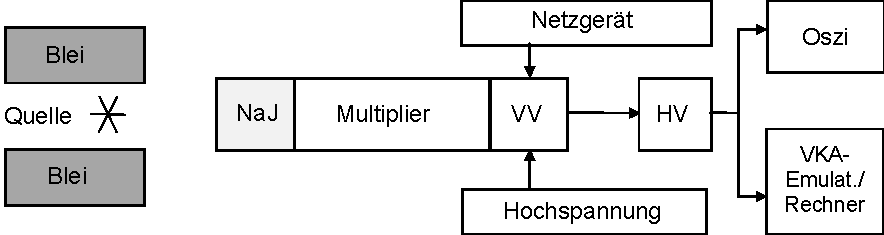
\includegraphics[width=.8\textwidth]{images/aufbau.pdf}
\caption{Schematischer Aufbau des Versuchs \cite{wiki} mit NaJ-Detektor, VV-Vorverstärker, HV-Hauptverstärker, VKA-Vielkanalanalysator}
\label{fig:aufbau}
\end{figure*}

\subsection{Ablauf}

\section{Auswertung}


\newpage
\bibliographystyle{unsrtnat}
\bibliography{raybib}

\end{document}





